
En esta segunda actividad practica nos centraremos en la correccion radiometrica
de imagenes satelitales. Son objetivos de la misma

\begin{itemize}
    \item Poder abrir una imagen satelital desde el metadato.
    \item Convertir los valores de la imagen a reflectancia tope de la
        atmosfera.
    \item Corregir la imagen satelital utilizando los metodos de \emph{dos} y
        \emph{cost}
    \item Corregir la imagen satelital utilizando el \emph{6S web}
\end{itemize}

\subsection{Calculo de reflectancia a tope de la atmosfera}

Para poder convertir una imagen a reflectancia a tope de la atmosfera vamos a
necesitar no solo la imagen sino tambien la informacion adicional sobre la misma
incluida en el metadato.

Para abrir una imagen satelital desde el metadato utilizaremos las funciones
disponibles en \texttt{RStoolbox}. Dicho paquete incluye diversar herramientas
para trabajar con sensores remotos y ya lo utilizamos antes para graficar
imagenes satelitales.

\begin{exa}
   Comencemos analizando un ejemplo sencillo, abriremos una imagen landsat 7 
    desde el metadato y la mostraremos en combinacion de bandas de falso color
    compuesto, ademas de analizar las propiedades basicas de la misma.
    \begin{lstlisting}
    meta.2000 <- readMeta("raster_data/LE72240782000188EDC00/LE72240782000188EDC00_MTL.txt")
    \end{lstlisting}
    Podemos mostrar las distintas variables incluidas en el objeto usando el
    signo \$ y el nombre de la misma. Por ejemplo
    \begin{lstlisting}
    meta.2000$SOLAR_PARAMETERS
    \end{lstlisting}
    da como resultado
    \begin{Verbatim}[fontsize=\small]
     azimuth elevation  distance 
    37.38251  31.14409   1.01670 
    \end{Verbatim}
    A partir del metadato podemos cargar la imagen completa con el comando
    \texttt{stackMeta}. Ademas eliminaremos en este caso las bandas 6 y 7 por
    ser termicas.
    \begin{lstlisting}
    dn.2000 <- stackMeta(meta.2000)
    dn.2000 <- dn.2000[[-6:-7,]]
    dn.2000
    \end{lstlisting}
    obtenemos como resultado un objeto raster stack
    \begin{Verbatim}[fontsize=\small]
    class       : RasterStack 
    dimensions  : 2412, 1834, 4423608, 6  (nrow, ncol, ncell, nlayers)
    resolution  : 30.00402, 30.00265  (x, y)
    extent      : 731118.6, 786146, 7101531, 7173897  (xmin, xmax, ymin, ymax)
    coord. ref. : +proj=utm +zone=21 +south +datum=WGS84 +units=m +no_defs
                  +ellps=WGS84 +towgs84=0,0,0 
    names       : B1_dn, B2_dn, B3_dn, B4_dn, B5_dn, B7_dn 
    min values  :     0,     0,     0,     0,     0,     0 
    max values  :   255,   255,   255,   255,   255,   255 
    \end{Verbatim}
    y podemos mostrar la iamgen como hicimos antes
    \begin{lstlisting}
    plotRGB(dn.2000, r=3, g=2, b=1, stretch="lin")
    \end{lstlisting}

     \begin{figure}
     \begin{center}
         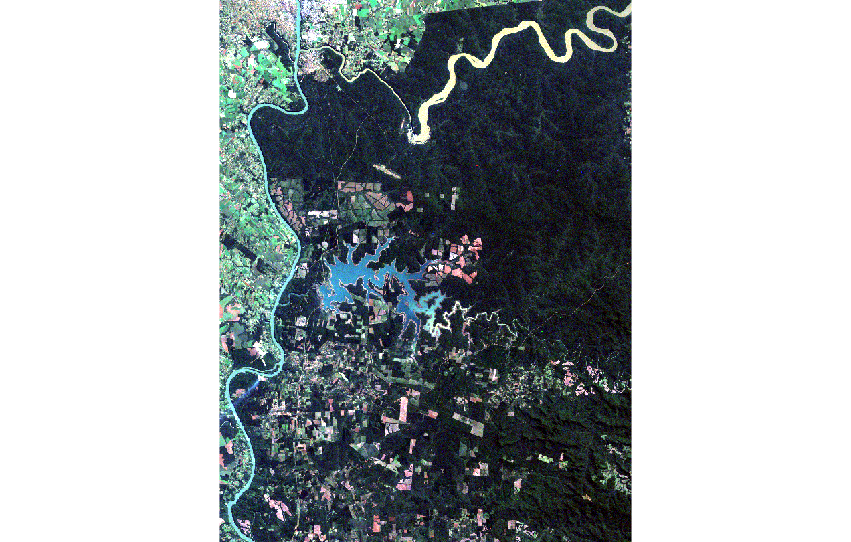
\includegraphics[scale=0.6]{dn-l7-rgb}
     \end{center}
     \caption{Imagen en combinacion color real de la zona de interes sobre la
         imagen en DN Landsat 7.}
     \label{fig:dn-l7-rgb}
     \end{figure}
\end{exa}

De esta forma podemos tener el archivo cargado en DN con todos sus metadatos
para convertirlo a reflectancia. Para pasar nuestra imagen a reflectancia a tope
de la atmosfera tenemos dos maneras de hacerlo. Podemos hacerlo a mano
utilizando las herramientas algebraicas de R o podemos hacerlo con la funcion
especifica de \texttt{RStoolbox}.

\begin{exa}
    Veamos como realizar el calculo de reflectancia a tope de la atmosfera
    utilizando el metadato paso por paso

    \begin{lstlisting}
    dn2ref.2000 <- meta.2000$CALREF[1:6,]
    elev.2000 <- pi*meta.2000$SOLAR_PARAMETERS['elevation']/180
    \end{lstlisting}
    extraemos primero del metadatos los parametros de calibracion en
    reflectancia y el angulo de elevacion solar.
    \begin{lstlisting}
    toam.2000 <- (dn.2000*dn2ref.2000$gain+dn2ref.2000$offset)/sin(elev.2000)
    names(toam.2000) <- c("blue","green","red","nir","swir1","swir2")
    \end{lstlisting}
    Convertimos luego la imagen a reflectancia y la dividimos luego por el
    angulo solar. Luego cambiamos los nombres de las bandas

    Otra forma forma de realizar este proceso es utilizando la funcion
    \texttt{radCor}. En este caso debemos dar la imagen en DN, el metadato y
    cual es la cantidad que queremos calcular.

    \begin{lstlisting}
    toa.2000 <- radCor(dn.2000, metaData = meta.2000, method = "apref")
    \end{lstlisting}

    podemos comparar los resultados de ambos metodos inspeccionando los objetos.
    \begin{lstlisting}
    toam.2000 
    \end{lstlisting}
    \begin{Verbatim}[fontsize=\small]
    class       : RasterBrick 
    dimensions  : 2412, 1834, 4423608, 6  (nrow, ncol, ncell, nlayers)
    resolution  : 30.00402, 30.00265  (x, y)
    extent      : 731118.6, 786146, 7101531, 7173897  (xmin, xmax, ymin, ymax)
    coord. ref. : +proj=utm +zone=21 +south +datum=WGS84 +units=m +no_defs
                  +ellps=WGS84 +towgs84=0,0,0 
    data source : in memory
    names       :        blue,       green,         red,         nir,    swir1,       swir2 
    min values  : -0.01976113, -0.02181530, -0.02029439,  0.01934678,    -0.02781926, -0.02678077 
    max values  :   0.6106812,   0.5609009,   0.6079443,   0.8696885,    0.8640919,   0.8263815 
    \end{Verbatim}
    \begin{lstlisting}
    toa.2000 
    \end{lstlisting}
    \begin{Verbatim}[fontsize=\small]
    class       : RasterStack 
    dimensions  : 2412, 1834, 4423608, 6  (nrow, ncol, ncell, nlayers)
    resolution  : 30.00402, 30.00265  (x, y)
    extent      : 731118.6, 786146, 7101531, 7173897  (xmin, xmax, ymin, ymax)
    coord. ref. : +proj=utm +zone=21 +south +datum=WGS84 +units=m +no_defs
                  +ellps=WGS84 +towgs84=0,0,0 
    names       :     B1_tre,     B2_tre,     B3_tre,     B4_tre,     B5_tre,    B7_tre 
    min values  : 0.00000000, 0.00000000, 0.00000000, 0.01934678, 0.00000000,    0.00000000 
    max values  :  0.6106812,  0.5609009,  0.6079443,  0.8696885,  0.8640919,    0.8263815 
    \end{Verbatim}
    vemos algunas diferencias entre ambas funciones. Por ejemplo las
    reflectancias minimas no pueden ser negativas y la funcion \texttt{radCor}
    contempla esto. De esta forma hemos obtenido a reflectancia a tope de la
    atmosfera a partir del metadato.
    \end{exa}

\begin{act}
    Inspeccione la reflectancia a tope de la atmosfera para todas las bandas.
    Para esto realice los histogramas, graficos de dispersion, calcule la media,
    el desvio standar y cualquier otra medida estadistica que le guste.
\end{act}
\subsection{Calculo de reflectancia corregida atmosfericamente}

La funcion \texttt{radCor} dispone distintos parametros para hacer distintos
tipos de correcciones atmosfericas. Ya vimos \emph{apref} que nos permitio
calcular la reflectancia a tope de la atmosfera. Veamos como aplicar el metodo
de substraccion de cuerpo obscuro.

\begin{exa}
    Apliquemos el metodo de simple dos para corregir la imagen. En este caso
    solamente restaremos el minimo en cada banda a la imagen para las bandas
    donde existe haze, es decir en la zona del visible y del infrarrojo.

    En R esto se hace en dos pasos. Estimamos el haze con el primer comanzo y
    corregimos la imagen con el segundo.
    \begin{lstlisting}
    haze.2000 <- estimateHaze(dn.2000,darkProp = 0.01, hazeBands = 1:4, plot=TRUE)
    sdos.2000 <- radCor(dn.2000, metaData = meta.2000, 
                 hazeValues = haze.2000,
                 hazeBands = c("B1_dn","B2_dn","B3_dn","B4_dn"), 
                 method="sdos")
    \end{lstlisting}
    en este caso los valores de haze estimados son
    \begin{Verbatim}[fontsize=\small]
    B1_dn B2_dn B3_dn B4_dn 
       41    27    20    15 
    \end{Verbatim}
    Para hacer un analisis de lo que pasa en la situacion, vamos a graficar los
    histogramas de cada banda para la imagen en reflectancia TOA y corregida por
    el metodo simple dos. Para esto usaremos el paquete \texttt{rasterVis}
    \begin{lstlisting}
    B1 <- densityplot(~B1_tre+B1_sre, data=toa.boa, xlab="Reflectancia",
                      ylab="", main="Banda azul", plot.points=FALSE, xlim=c(0,0.3),
                      key=simpleKey(text=c("Tope de la atmosfera",
                                           "Correccion Simple DOS"),
                                           lines=TRUE, points=FALSE))    
    B2 <- densityplot(~B2_tre+B2_sre, data=toa.boa, xlab="Reflectancia",
                      ylab="", main="Banda verde", plot.points=FALSE, xlim=c(0,0.3),
                      key=simpleKey(text=c("Tope de la atmosfera",
                                           "Correccion Simple DOS"),
                                           lines=TRUE, points=FALSE))    
    B3 <- densityplot(~B3_tre+B3_sre, data=toa.boa, xlab="Reflectancia",
                      ylab="", main="Banda roja", plot.points=FALSE, xlim=c(0,0.3),
                      key=simpleKey(text=c("Tope de la atmosfera",
                                           "Correccion Simple DOS"),
                                           lines=TRUE, points=FALSE))    
    B4 <- densityplot(~B4_tre+B4_sre, data=toa.boa, xlab="Reflectancia",
                      ylab="", main="Banda nir", plot.points=FALSE, xlim=c(0,0.3),
                      key=simpleKey(text=c("Tope de la atmosfera",
                                           "Correccion Simple DOS"),
                                           lines=TRUE, points=FALSE))    
     print(B1,split = c(1, 1, 2, 2),more=TRUE)
     print(B2,split = c(2, 1, 2, 2),more=TRUE)
     print(B3,split = c(1, 2, 2, 2),more=TRUE)
     print(B4,split = c(2, 2, 2, 2),more=FALSE)
    \end{lstlisting}
    En este caso las primeras 4 funciones crean los histogramas para cada banda
    corregida mientras que las ultimas 4 lineas los imprimen en una grilla.
    \begin{figure}
    \begin{center}
        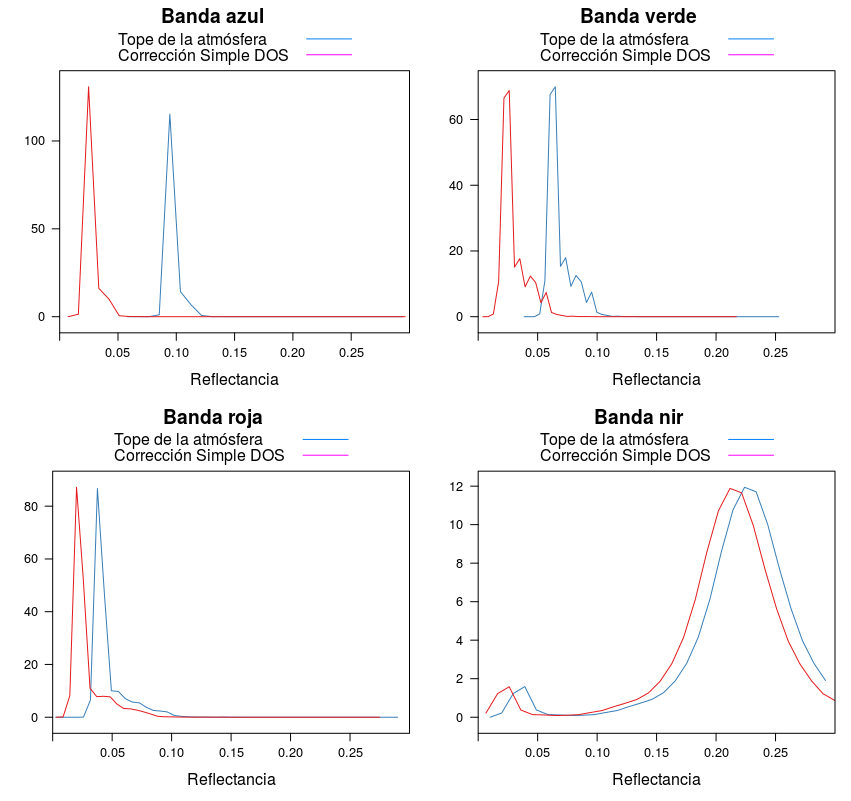
\includegraphics[scale=0.6]{simpledos.png}
    \end{center}
    \caption{Graficos de los histogramas para las distintas bandas donde se
        muestra el nivel de correccion en cada una.}
    \label{fig:simpledos.png}
    Notamos en este casoq ue la correccion se vuelve menos importante a medida
        que crece la longitud de onda.
    \end{figure}
    
\end{exa}
\begin{act}
    Analice los valores de haze obtenidos por la funcion stimate hace y en caso
    de que sea necesario, corrijalos para la banda indicada.
\end{act}

\begin{act}
    Utilice el metodo \emph{costz} para corregir la imagen a reflectancia a tope
    de la superficie.
\end{act}

\begin{act}
    Guarde los archivos raser generado por cada uno de los metodos de
    correccion. Abralos en qgis y comparelos visualmente.    
\end{act}


\subsection{6S}
\label{sub:corr:6S}

Veamos ahora como operar con el 6S para obtener una estimacion de los parametros
atmosfericos. Para esto utilizaremos la version web del 6S que se encuentra
disponible en http://6s.ltdri.org/pages/run6SV.html.

Para utilizarla ingresaremos a la pagina y haremos click en el boton
\menu{Submit query}. Iremos luego configurando paso a paso nuestro modelo de la
atmosfera haciendo siempre luego click en el boton \menu{submit query} para
pasar al paso siguiente.

Los parametros para nuestro modelo son

\begin{enumerate}
    \item Geometrical conditions
        \begin{itemize}
            \item TM (Landsat)
            \item Month: 4, Day:13, GTM decimal hour: 13.60, Longitude:
                -63.8606, Latitude: -24.9937.
        \end{itemize}
    \item Atmospheric Model
        \begin{itemize}
            \item Select Atmospheric Profile: Mid latitude summer
            \item Select aerosol model: Continental Model
            \item Visibility: 60
        \end{itemize}
    \item Target \& sensor altitude
        \begin{itemize}
            \item Select targe altitude: sea level
            \item Select sensor altitude: satellite level
        \end{itemize}
    \item Spectral conditions
        \begin{itemize}
            \item Select spectral conditions: choose band
            \item Select band: 1st band of tm (landat 5)
        \end{itemize}
    \item Ground reflectance
        \begin{itemize}
            \item Ground reflectance type: homogeneous surface
            \item Directional effect: no directional effect
            \item Specify surface reflectance: input constant value of ro
            \item input constant value for ro: 0
        \end{itemize}
    \item Signal
        \begin{itemize}
            \item Atmospheric correction mode: no atmospheric correction
        \end{itemize}
\end{enumerate}

En \menu{7.Results} podemos ver el resultado haciendo click en \emph{Output
file}. Del mismo debemos extraer los valores de
 \begin{itemize}
     \item \texttt{global gas. trans. - total}
     \item \texttt{total sca. trans. - total}
     \item \texttt{spherical albedo - total}
     \item \texttt{reflectance I - total}
 \end{itemize}

Una vez ejecutado el proceso puede usarse el siguiente codigo para corregir
todas las bandas utilizando R.

\begin{lstlisting}
    a <- c(0.98,0.90,...) # Global gas transmitance
    b <- c(0.81,0.90,...) # Total scatering transmitance
    g <- c(0.15,0.10,...) # Spherical albedo
    r <- c(0.08,0.05,...) # Reflectance I
    sss.2000 <- (toa.2000/(a*b)-r/b)/(1+g*(toa.2000/(a*b)-r/b))
\end{lstlisting}


\begin{act}
    Realice una extraccion de firmas espectrales para distintass coberturass de
    cada uno de los archivos raster obtenidos y grafiquelos en el mismo grafico.
    Comparela con la firma espectral obtenida a partir de la imagen corregida
    por el usgs.
\end{act}

\begin{act}
    Haga un grafico de densidades que muestre los distintos metodos de
    correccion atmosfericos para cada banda.
\end{act}
